\chapter{\textbf{RESULTS AND DISCUSSION}}
To illustrate the applicability of the three-band \ac{TBM} developed in Chapter~3, we consider the case of monolayer MoS$_{2}$ as a representive example of \acp{TMD}. For completeness, similar calculations have been perfomed for other \ac{TMD} monolayers. The corresponding results are provided in \hyperref[appendix B]{Appendix~B}.
\section{Band structure of MoS$_{2}$ at zero magnetic field}
We begin the analysis by calculating the band structure of monolayer MoS$_2$ using the three-band tight-binding model that includes spin–orbit coupling (SOC). This model captures the essential features of the low-energy physics near the $K$ and $K'$ points of the Brillouin zone.

By solving the Hamiltonian in Eq.~(3.11), we obtain the eigenvalues of the Hamiltonian, which are evaluated across the entire Brillouin zone. These are computed over all $k$-points throughout the entire \ac{BZ}, and the corresponding band structure is illustrated in Fig.~4.1. The presence of three orbitals from the M atom in the unit cell results in three energy bands: one \ac{VB} and two \acp{CB}. When spin–orbit coupling is included, these bands split due to spin degeneracy, leading to six bands in total. Among them, the \ac{VB} exhibits a prominent spin splitting near the $K$ and $K'$ points, while the \acp{CB} remain nearly degenerate.


%The diagram in Fig. 2.8 shows the significant splitting of the valence bands at the $K$ and $K'$ points of MoS$_{2}$, caused by the \ac{SOC}, with a value of $\Delta_{\text{SOC}}^{\lambda} = 2 \lambda = 146$ meV. Although the \ac{NN} \ac{TB} model is not accurate as the TNN one, it can be seen that the \ac{NN} \ac{TB} bands agree well the \ac{TNN} results near the $K$ and $K'$ points.

This splitting is attributed to the atomic \ac{SOC} of the Mo atom, with a magnitude of $\Delta_{\text{SOC}}^{\lambda} = 2\lambda = 146$ meV. This effect is a hallmark of monolayer \acp{TMD}, playing a crucial role in spin–valley coupling and valley-selective optical properties.


\begin{figure*}[htb]
\begin{subfigure}[b]{0.495\textwidth}
	\centering
	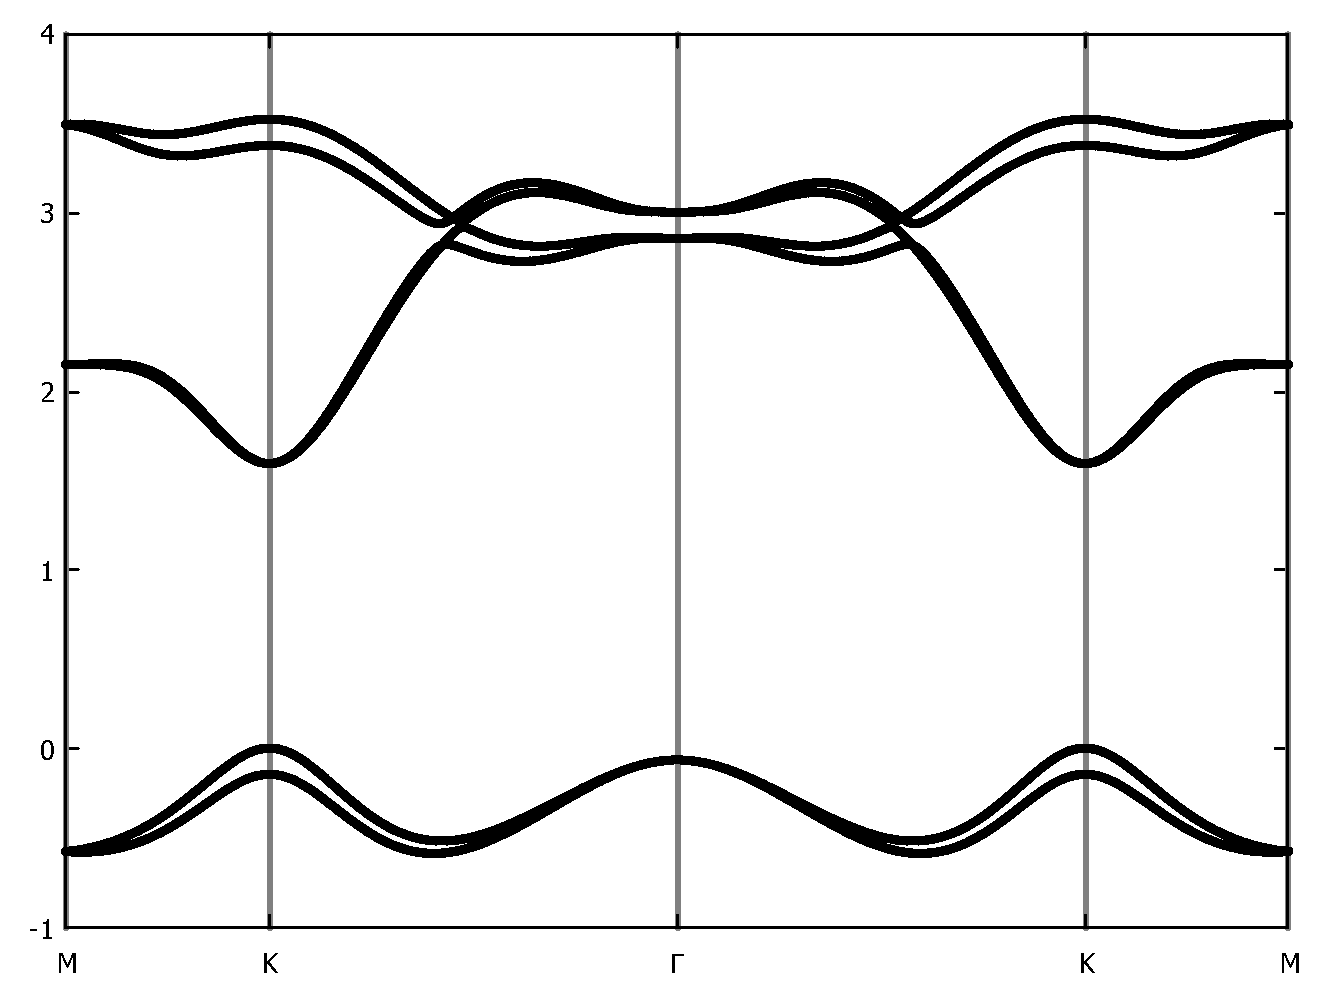
\includegraphics[width=\linewidth]{pic/bandstructureSOC.pdf}
	%\caption{\label{band structure SOC}}
\end{subfigure}
\begin{subfigure}[b]{0.495\textwidth}
	\centering
	\includegraphics[width=\linewidth]{pic/bandstructureSOCTNN.pdf}
	%\caption{\label{HB SOC}}
\end{subfigure}
\caption[Banstructure of NN and TNN monolayer MoS$_{2}$ with SOC without magnetic field.]{The band structure of monolayer MoS$_2$ in the absence of a magnetic field along the $\Gamma$–K direction exhibits significant spin splittings at the $K$ and $-K$ points, primarily due to spin–orbit coupling (SOC). Figures 4.1(a) and 4.1(b) show the results obtained using \ac{NN} and \ac{TNN} model, respectively.
}
\end{figure*}
\section{Hofstadter butterfly of monolayer MoS$_{2}$}
In this section, we explore the Hofstadter spectrum by presents the solution of Eq.~3.35. By plotting the band energies while varying the $p$, we obtain the famous Hofstadter butterfly \cite{PhysRevB.14.2239}, a complex fractal structure as seen in Fig.~4.2. This fractal spectrum is a result of two competing effects, lattice periodicity and magnectic unit cell periodicity enforced by the presence of the magnetic field. The magnetic field enters the \ac{TB} Hamiltonian only through the fraction $p/q$, which is proportional to the magnetic flux through the primitive unit cell of the lattice. In general, as the lattice geometry evolves, the area of the primitive unit cell changes $m$ times.

In this study, the Hofstadter butterfly of MoS$_2$ is generated at the $K$-point. Additionally, we compute a single-band Hofstadter butterfly (using only the conduction band) to highlight the underlying triangular lattice structure of MoS$_2$. In Fig.~4.2, for the \ac{NN} model, the Hofstadter butterfly structure clearly resembles that of a triangular lattice, as previously reported in other materials such as \cite{li2011}.


\begin{figure*}[htb]
\centering
\begin{subfigure}[b]{0.32\textwidth}
	\centering
	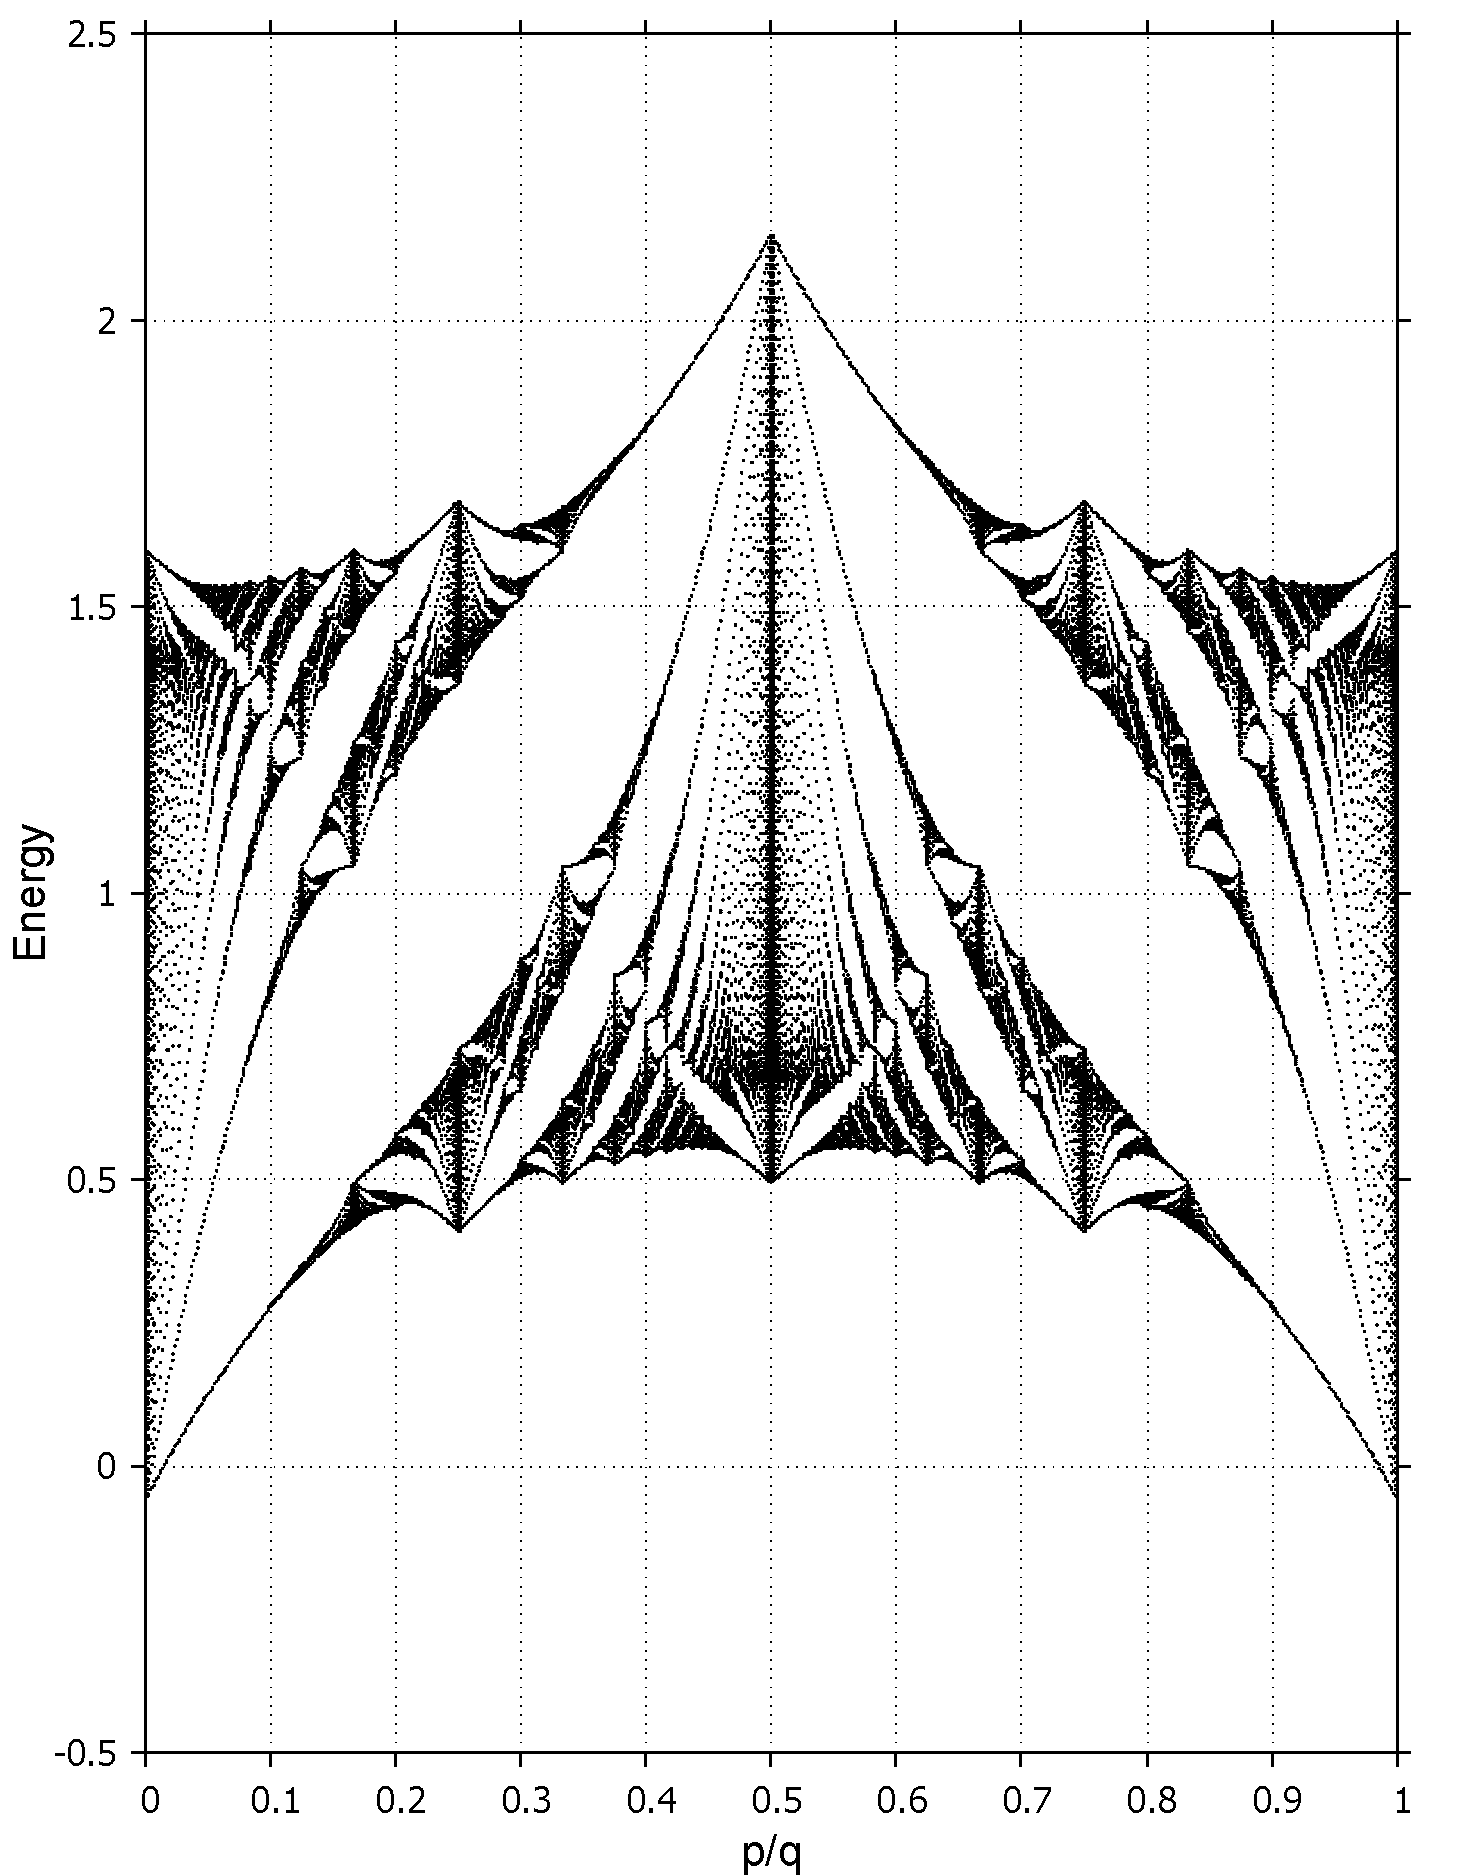
\includegraphics[width=0.95\textwidth,height=1.2\linewidth]{pic/h0_tam giac_q_797.png}
	\label{fig:3 band}
\end{subfigure}
\begin{subfigure}[b]{0.32\textwidth}
	\centering
	\includegraphics[width=0.95\textwidth,height=1.2\linewidth]{pic/h0_tam giac_TNN_LDA_q_797.png}
	\label{}
\end{subfigure}
\begin{subfigure}[b]{0.32\textwidth}
	\centering
	\includegraphics[width=0.95\textwidth,height=1.2\linewidth]{pic/h0_tam giac_TNN_GGA_q_797.png}
	\label{}
\end{subfigure}
\begin{subfigure}[b]{0.32\textwidth}
	\centering
	\includegraphics[width=0.95\textwidth,height=1.2\linewidth]{pic/3band_gnuplot_TNN_q_797.png}
	\label{fig:1 band}
\end{subfigure}
\begin{subfigure}[b]{0.32\textwidth}
	\centering
	\includegraphics[width=0.95\textwidth,height=1.2\linewidth]{pic/3band_gnuplot_TNN_LDA_q_797.png}
	\label{}
\end{subfigure}
\begin{subfigure}[b]{0.32\textwidth}
	\centering
	\includegraphics[width=0.95\textwidth,height=1.2\linewidth]{pic/3band_gnuplot_TNN_GGA_q_797.png}
	\label{}
\end{subfigure}
\caption[Hofstadter butterfly for {TMD}.]{
	Hofstadter butterfly for single-band $\ket{dz} \equiv \ket{\phi_{1}^{1}(x,y)}$(a,b,c) and all band(d,e,f) for \ac{NN} and \ac{TNN} for MoS$_2$, respectively, with $q = 797$ and vary $p$ from 1 to $q$ with field strength $B_{0} = 4.6928 \times 10^{4}$ T. Here on $x-$axis represents the flux in units of quantum flux enclosed by the unit cell and $y-$axis represents the Energy. While (b,e) use \ac{GGA} parameter, (c,f) use \ac{LDA} one.
}
\end{figure*}

Another observation is that the lattice constant $a$ and the magnetic field $B$ always appears together in an expression with the magnetic field ($\tfrac{Ba^{2}\sqrt{3}}{2}$). This quantity reflects the flux per plaquette in the super magnetic unit cell, which is relevant is the context of Aharonov-Bohm effect \cite{aharonov1959}. Since the expression involves the product $Ba^{2}$, this implies that increasing $B$ by a certain amount is mathematically equivalent to increasing $a$. In other words, for energy calculations, increasing the strength of the magnetic field is physically equivalent to increasing the lattice constant, as both affect the system in the same way through the flux per unit cell. In addition, the three-band spectrum contains a complex and rich physics insight but it seem remains the fractal structure. The main energy bands are basically \acp{LL}, which we shall discuss in the next Section. For small values of the magnetic flux ratio $p/q$, these \acp{LL} manifest sharp and well-separated energy bands. However, when increasing $p$ from 1 to $q$, each \acp{LL} go a recursive splitting into $2q$ subbands. This structure arises from the magnetic unit cell's periodicity.

The spectrum exhibits several noticeable symmetries. First, it depends only on the flux ratio $p/q$, meaning that shifting $p/q$ by an integer $c$ (i.e., $p/q \rightarrow p/q + c$) leaves the spectrum unchanged. Additionally, the spectrum remains invariant under the transformation $p/q \rightarrow -p/q$, since if $\psi$ is an eigenstate with energy $E$ for flux $p/q$, its complex conjugate $\psi^*$ is an eigenstate with the same energy for flux $-p/q$. These two symmetries are general and not specific to the MoS$_{2}$ case. However, the third symmetry involves changing $p/q$ to $p/q + 1/2$, which is equivalent to flipping the sign of the hopping energies $t_{i}$ (i.e., $t_{i} \rightarrow -t_{i}$), resulting in an inversion of the spectrum, which is concealed clearly in square lattice \cite{PhysRevB.14.2239} or honeycomb lattice \cite{rammal1985}. In contrast, for the case MoS$_{2}$, the flux going through a unit cell is already one half, making this symmetry hidden. In fact, by adding an integer $n$ to the Peierls phase, one can effectively recover this symmetry, but this modification does not correspond to any physical observable.

\begin{figure*}[htb]
	\begin{subfigure}[b]{0.495\textwidth}
		\centering
		\includegraphics[width=\linewidth]{pic/plotHofstadterButterfly_q=797_MoS2_SOC_f.png}
		%\caption{\label{band structure SOC}}
	\end{subfigure}
	\begin{subfigure}[b]{0.495\textwidth}
		\centering
		\includegraphics[width=\linewidth]{pic/plotHofstadterButterfly_q=797_MoS2_SOC_LDA.png}
		%\caption{\label{HB SOC}}
	\end{subfigure}
	\caption[Hofstadter butterfly of monolayer MoS$_{2}$ with SOC in the presence of magnetic field.]{Hofstadter butterfly of monolayer MoS$_{2}$ with SOC at $K$ point. Figures 4.3(a) and 4.3(b) show the results obtained using \ac{NN} and \ac{TNN} model, respectively. }
\end{figure*}

The role of the eight hopping constants $t$ is just to set an energy scale. Change the hopping constants amounts to stretching the butterfly spectrum vertically, which is an overall scaling to the energy levels. Thus it does not give rise to any interesting physical phenomenon.

At the very large magnetic fields, the magnetic strength overwhelms the effects of \ac{SOC}. In this work, we treat the \ac{SOC} interaction as an adjustable constant in the Hamiltonian. As a result, the \ac{SOC} induces a spin splitting in the Hofstadter spectrum, see in Fig.~4.3.

In the case of the \ac{NN} model for MoS$_{2}$, our results are consistent with those reported in Refs.~\cite{ho2014,ho2015}. However, it is worth noting that our approach is more general, as Eq.~(3.34) explicitly incorporates the variation of $\delta_{n,n'}$, which was not considered in their formulation, such as in the equations of Refs.~\cite{ho2015} or Eq.~5 of Refs.~\cite{ho2014}. In addition, we also take into account interactions with 18 neighboring atoms, a level of detail that, to the best of our knowledge, has not been included in earlier models. This extended consideration significantly increases the computational complexity and demands.



\section{Landau levels in monolayer MoS$_{2}$}
The approach in Section~2.3 is for free electrons, but near the bottom of the two-dimensional tight-binding band of \ac{TMD} we must find a regime in which the electron behaves as a nearly one(At least with a nearly free dispersion relation). 

Recalling the result obtained for the dispersion relation of an electron within the \ac{TBM}
\begin{gather}
H_{11} = 2 t_{0} (\cos 2\alpha + 2 \cos \alpha \cos \beta) + \epsilon_{1}.
\end{gather}
The dispersion energy is approximately free-electron-like by Taylor expansion to second order of $\mathbf{k}$
\begin{equation}
\begin{aligned}
	H_{11}(\mathbf{k})
	& \approx 2 t_{0} \left[1 - \frac{a^{2} k_{x}^{2}}{2} + 2\left(1 - \f{a^{2} k_{x}^{2}}{8}\right)\left(1 - \f{3a^{2} k_{y}^{2}}{8}\right)\right] \\
	& = t_{0} \f{3}{16} \left(32 + a^{4} k_{x}^{2} k_{y}^{2}\right) - t_{0} \f{3}{2} a^{2}\left(k_{x}^{2} + k_{y}^{2}\right) + \epsilon_{1} ,
\end{aligned}
\end{equation}
the term $a^{4}$ is negligibly small, then we have
\begin{equation}
\begin{aligned}
	H_{11}(\mathbf{k})
	& \approx 6 t_{0} - \f{3}{2} t_{0} a^{2} (k_{x}^{2} + k_{y}^{2}) + \epsilon_{1}.
\end{aligned}
\end{equation}
One of the ways derivation of effective mass $m^{*}$ is substitution $\hbar\mathbf{k} \rightarrow \mathbf{\Pi} + e \mathbf{A}$, with Landau gauge $\mathbf{A} = (0,Bx,0)$
\begin{equation}
\begin{aligned}
	H_{11}(\mathbf{\Pi})
	& \approx 6 t_{0} - \f{3}{2} t_{0} \f{a^{2}}{\hbar^{2}} \left[ \Pi_{x}^{2} + \left(\Pi_{y} + e B x\right)^{2}\right] + \epsilon_{1}                                                           \\
	& \approx 6 t_{0} - \f{3}{2} t_{0} \f{a^{2}}{\hbar^{2}} \Pi_{x}^{2} - \f{3}{2} t_{0} \f{a^{2}}{\hbar^{2}} (e B)^{2} \left[ x - \left(- \f{\hbar k_{y}}{eB}\right) \right]^{2} + \epsilon_{1}.
\end{aligned}
\end{equation}
The Eq (4.4) can be rewrite in the form as
\begin{gather}
E(\mathbf{\Pi}) = 6 t_{0} - \left[\f{1}{2m^{*}} \Pi_{x}^{2} + \f{1}{2} m^{*} \omega_{c}^{2}(x - x_{0})^{2}\right] + \epsilon_{1},
\end{gather}
where $m^{*} = \frac{\hbar^{2}}{3t_{0}a^{2}}$ is the effective mass and $x_{0} = \frac{\hbar k_{y}}{eB}$. Subsequently, the cyclotron frequency is
\begin{gather}
\omega_{c} = \f{eB}{m^{*}} = \f{8 \pi \sqrt{3} t_{0}}{\hbar}  \f{p}{q},
\end{gather}
and therefore the Landau levels near the bottom of the band structure can be written as
\begin{equation}
\begin{aligned}
	E_{n}
	& = 6 t_{0} - \hbar \omega_{c} (n + 1 /2) + \epsilon_{1}                    \\
	& = t_{0} \left(6 - 8\pi\sqrt{3} \f{p}{q}( n + 1 /2)\right) + \epsilon_{1},
\end{aligned}
\end{equation}
in linear order of an uniform-flux, where $n$ is Landau index. 

\begin{figure*}[htb]
\centering
\begin{subfigure}[b]{0.49\textwidth}
	\centering
	{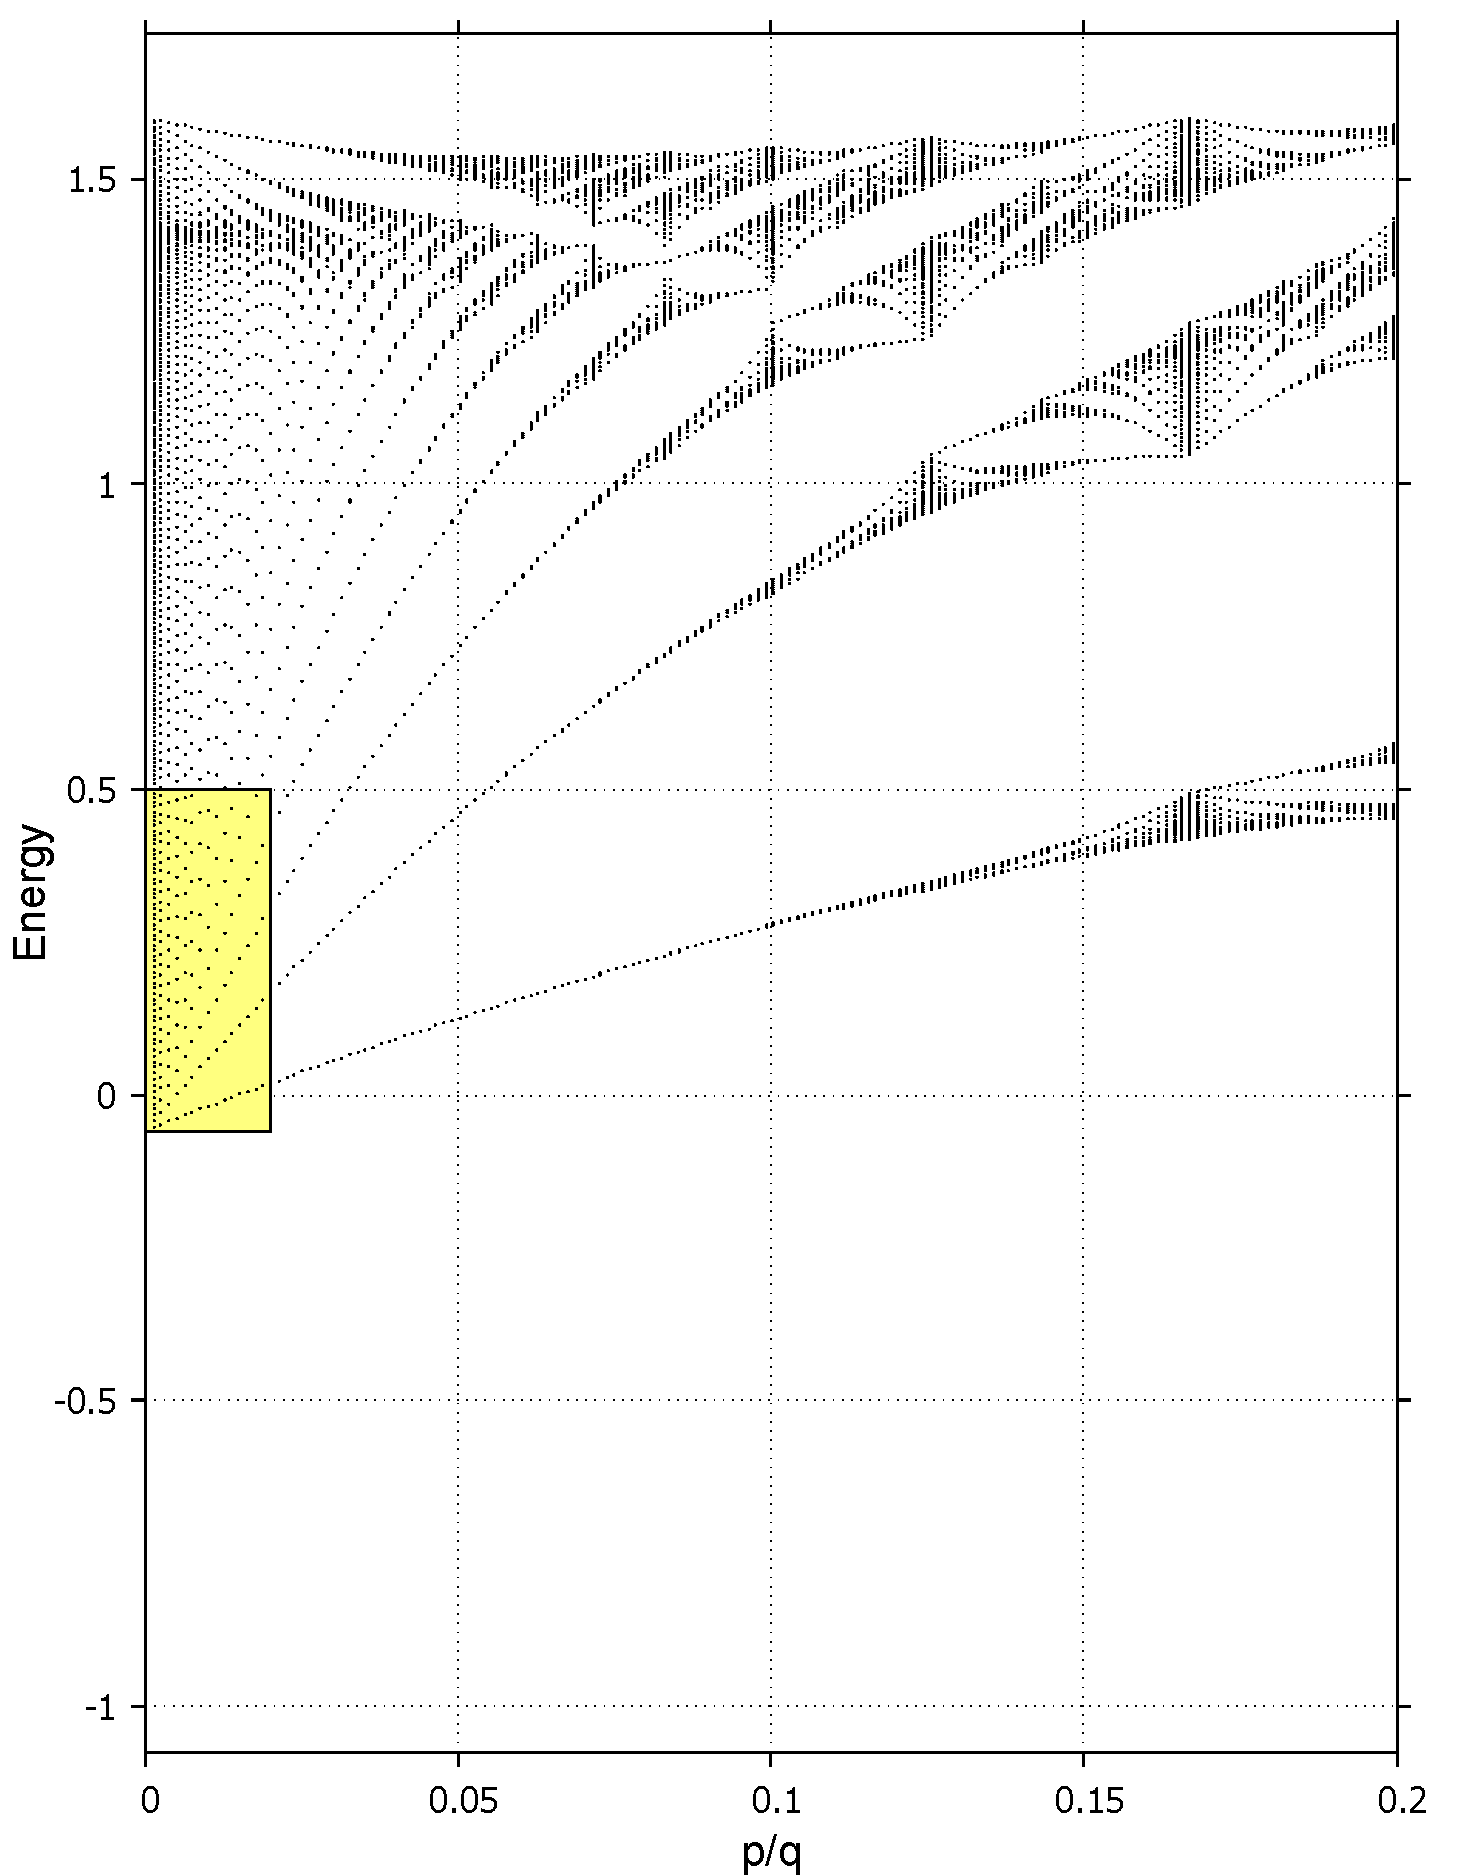
\includegraphics[width=0.85\textwidth,height=1.2\linewidth]{pic/small_area_LL.png}}
\end{subfigure}
\begin{subfigure}[b]{0.49\textwidth}
	\centering
	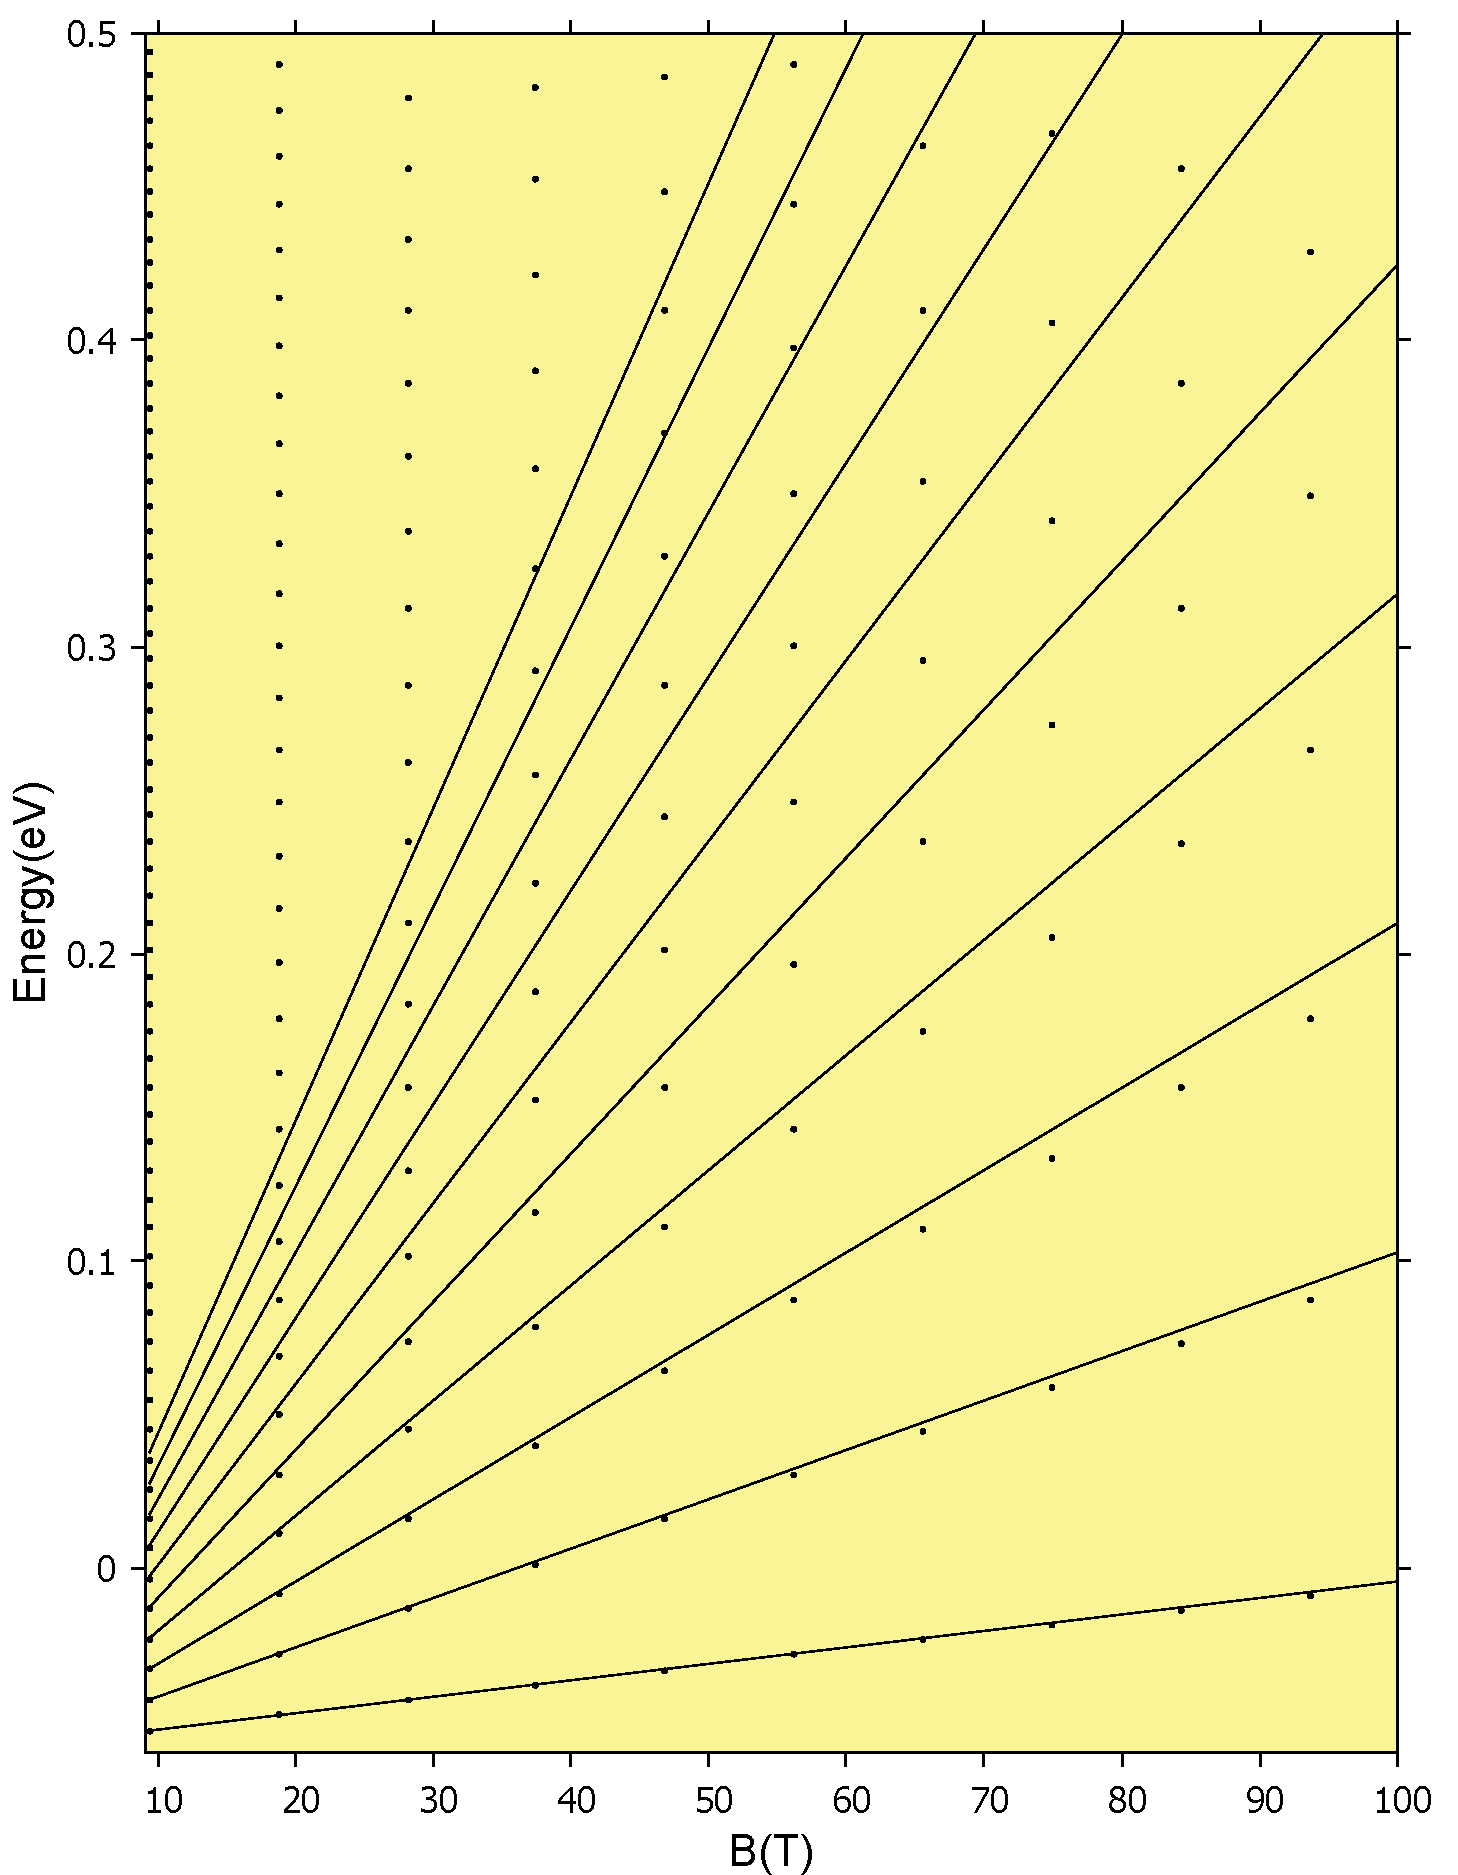
\includegraphics[width=0.85\textwidth,height=1.2\linewidth]{pic/landaulevel_h0_q_797.pdf}
\end{subfigure}
\caption[Landau levels in Hofstadter butterfly.]{
	(a) Same plot as Fig.~4.4(a) but considering a small area and (b) shows both the Landau fan diagram and the Hofstadter butterfly. Display the first $n = 30$ levels near the bottom of the conduction band for a magnetic field up to $B = 500$ T.
}
\end{figure*}

In Fig.~4.4 we compare the spectrum of a small section of single-band with $p / q = 1 / 797$, which is equivalent to small magnetic field, the spectrum of MoS$_{2}$, with the energy of Landau levels given by Eq.~(4.7) show standard equally spaced \acp{LL} \cite{Shoenberg_1984,singleton2001band,blundell2001magnetism,kittel1987quantum} near the bottom of the bands, as plotted in Fig.~4.4(b). The fan of \acp{LL} can be clearly seen emergin from the pattern in Fig.~4.4(a).

In Fig.~4.4(a), there is just single-band in case zero field, with the effective mass $m^{*} = \frac{\hbar}{3 t_{0} a^{2}}$. The numerical result for this portion of the spectrum are shown in Fig.~4.4 for $p/q \geq 1/797$. The first few \acp{LL} are clearly seen, and the asymtotic slopes $p/q$ at large $q$ given by Eq.~(4.7) are shown for comparison for the first five Landau levels at $B \leq 100$ T. At the values of $B$ the fit is not ideal, but it does seem to be improving with the decreasing $p/q$.

Figure~4.4 also displays a blowup of the low uniform magnetic field region, showing the \acp{LL} as a function of $\Phi / \Phi_{0}$. These Landau levels appear approximately linear in $B$, which is a consequence of magnetic quantization of the parabolic bands at $B = 0$~T. As the magnetic field increases, the \acp{LL} are sequentially depopulated. For example, at $B = 200$~T, the levels are completely filled up to $n = 4$, whereas at $B = 500$~T, only levels up to $n = 1$ remain filled, and higher levels are emptied. When compared with the theoretical study presented in Section~2.3, we find that the Hofstadter butterfly in the weak magnetic field regime is in excellent agreement with the predicted Landau level structure. This indicates that the model accurately captures the low-field physics.


\section{Color the Hofstadter butterfly}
In Section~2.4.2, we arrived at the Hall conductivity equation from a single subband, which is given by \cite{kohmoto1989,hatsugai1990energy,kohmoto1985topological,thouless1982}
\begin{gather}
\sigma_{xy} = \f{e^{2}}{h} \sum_{n}^{\text{occ.}} \f{1}{2\pi} \dps\oiint_{\text{{BZ}}} d k_{x} d k_{y} \Omega_{n}^{z} (\mathbf{k}).
\end{gather}
In general, the Berry curvature intergrated over a closed manifold is quantized in the units of $e^{2} / h$ and equals to the net number of monopoles inside. This number is called the Chern number and is responsible for a number of quantization effects. Therefore the Hall conductivity is quantized for a two dimensional band insulator of noninteracting electrons. By integrating the Berry curvature over the entire Brillouin zone, we arrived at the \ac{TKNN}'s formula \cite{thouless1982}
\begin{gather}
\sigma_{xy} = \f{e^{2}}{h} \nu, \quad \nu = 1,2,...
\end{gather}
$\nu$ is the Chern number.

%With the cyclotron frequency in Section 2.4, the electron energy is quantized to the Landau levels.

We, then, calculate the quantum Hall conductivity by the Streda formula \cite{streda1982}
\begin{gather}
\sigma_{xy}(B,E_{F}) = e \f{\partial N (E,B)}{\partial B} \at{E=E_{F}}{},
\end{gather}
%As show in Fig. (2.12), the Hall conductivity is quantized at colored points.
where $N(E_{F},B)$ is the number of state at fixed Fermi energy $E_{F}$. Combining Eq.~(4.9) and Eq.~(4.10), we have
\begin{gather}
	\f{\partial N}{\partial B} = \f{e}{h} \nu.	
\end{gather}
Assuming that $B$ vary slightly
\begin{gather}
	N = c + \f{e}{h}B \nu, \quad c \; \text{is constant}.
\end{gather}
Before this, we have defined $\frac{p}{q} = \frac{eBa^{2}\sqrt{3}}{2h}$, with $S = \frac{\sqrt{3} a^{2}}{2}$ is the area of the original unit cell in \hyperref[Section 3.2]{Section 3.2}. Multiply $S$ with Eq.~(4.12), we have
\begin{gather}
	N \times S = c + \f{p}{q} \nu,
\end{gather}
and the density of electron in a single band is given by $\frac{1}{Sq}$, thus when there are $r$ bands below the Fermi energy level, the density of electron for $r^{\text{th}}$ band is
\begin{gather}
	N = \f{r}{Sq}.
\end{gather}
Then, the Eq.~(4.13), is written as,
\begin{gather}
	r = c \times q + p \times \nu_{r},
\end{gather}
in this equation $r$, $q$, $p$, $\nu$ are integers, thus, $c\times q$ must be an integer. On the one hand, since $c$ is independent of $q$, then $c$ itself must be an integer, namely $s_{r}$. Thus we have
\begin{gather}
	r = q \times s_{r} + p \times \nu_{r},
\end{gather}
this equation is usually named as the Diophantine equation. While $\nu_{r}$ is the Chern number associated with the quantized Hall conductance which can be found by taking $\nu_{r}$ between $-q/2$ and $q/2$ and determining its allows conductance to be determined, $s$ is another integer that play a role in indentify the gap index.

The Hall conductivity of the lattice model for an electron in a background magnetic field can only be computed when the flux ratio $\frac{\Phi}{\Phi_{0}} = \frac{p}{q}$ is rational. In this case, we can use the TKNN formula, but with the Chern number, which used to be defined by intergrating over the Brillouin zone, now arising by intergrating over the magnetic Brillouin zone. Others derivation is in \cite{di2022linking,dana1985,avron2003}.

The Diophantine equation is crucial in understanding the quantization of Hall conductance in the Hofstadter butterfly. The Chern number $\nu$ determines the topological nature of the bands and their contribution to the Hall conductance, while the integer $s$ identifies specific energy gaps in the spectrum. These gaps are directly linked to incompressible quantum Hall states, which are of significant interest in both theoretical and experimental condensed matter physics. The solutions to the Diophantine equation are presented in Table D.1 in \hyperref[appendix D]{Appendix D}, revealing many interesting observations can be extracted from it. Firstly, we observe the occurence values of $\nu = \pm 1$ at both $r = p$ and $r = q-p$. This owing to each band being devided into $q$ subbands. Significantly, the case $r = p$, where the corresponding gap index naturally corresponds to the first gap in the Landau level. The second observation is the symmetry of the table, the value of $\nu_{r}$ is equal to $-\nu_{q-r}$. This is due, once again, to the symmetry of the butterfly.
\begin{figure*}[htb]
	\centering
	\begin{subfigure}[b]{0.495\textwidth}
		\centering
		{\includegraphics[width=\linewidth]{pic/1band_Chern_q_199_f.pdf}}
	\end{subfigure}
	\begin{subfigure}[b]{0.495\textwidth}
		\centering
		\includegraphics[width=\linewidth]{pic/3band_Chern_q_199_f.png}
	\end{subfigure}
	\caption{
		Colored points version of Hofstadter butterfly.
	}
\end{figure*}

To further explore the intricate fractal nature of the Hofstadter spectrum, we shall now achieve the colored Hofstadter butterfly. There are many ways to color the butterfly. For instance, a common approach is to color each point of the butterfly based on their Chern number, as illustrated in the Fig.~4.5. At these points, the Hall conductivity hightlights exactly quantization. However, a drawback of this method is that the butterfly may contain a dense of points, which can make it difficult to visualise fine details in the colored spectrum.

%	\begin{subfigure}[b]{0.495\textwidth}
%	\centering
%	\includegraphics[width=0.85\textwidth,height=1.2\linewidth]{pic/wannier_gnu.pdf}
%\end{subfigure}



%\begin{figure*}[htb]
%	\centering
%	\begin{subfigure}[b]{0.495\textwidth}
	%		\centering
	%		\includegraphics[width=\linewidth]{pic/1band_dataHofstadterButterfly_q_797_fix_chern.eps}
	%	\end{subfigure}
%	\begin{subfigure}[b]{0.495\textwidth}
	%		\centering
	%		\includegraphics[width=\linewidth]{pic/3band_Chern_q_797_colorplane2.png}
	%	\end{subfigure}
%	\caption[Colorplaned Hofstadter butterfly.]{
	%		q = 199 và q = 797. This color pallete was famously made by Avron\cite{avron2003}.
	%	}
%\end{figure*}
%\begin{figure*}[htb]
%	\centering
%	\begin{subfigure}[b]{0.495\textwidth}
	%		\centering
	%		\includegraphics[width=\linewidth]{pic/1band_Chern_q_797_colorplane.png}
	%	\end{subfigure}
%	\begin{subfigure}[b]{0.495\textwidth}
	%		\centering
	%		\includegraphics[width=\linewidth]{pic/3band_Chern_q_797_colorplane_f.png}
	%	\end{subfigure}
%	\caption[Colorplaned Hofstadter butterfly.]{
	%		q = 199 and q = 797. This color pallete was famously made by gnuplot.
	%	}
%\end{figure*}


Figures~4.6 and 4.7 displays the Hofstadter butterfly, color-coded according to the Hall conductance. Moreover, the number $p$ increases simultaneously with Chern number, making it challenging to maintain a fixed scale. Addressing this, we limit the Chern number scale within $-10 \leq \nu \leq 10$, any Chern number outside this range is set to zero. Regions with zero Hall conductance and the corresponding spectrum are left blank. Remarkably, the two largest gaps near the center of the figure are associated with small integers where the color coding accurately reflects their values. This idea was first made by Avron \textit{et al}\cite{avron2003}. 

\begin{figure*}[htb]
	\centering
	\begin{subfigure}[b]{0.495\textwidth}
		\centering
		{\includegraphics[width=\linewidth]{pic/1band_Chern_q_797_colorplane2.png}}
	\end{subfigure}
	\begin{subfigure}[b]{0.495\textwidth}
		\centering
		\includegraphics[width=\linewidth]{pic/3band_Chern_q_797_colorplane_f.png}
	\end{subfigure}
	\caption[Gaps color-coded Hofstadter butterfly for NN case.]{
		Gaps color-coded Hofstadter butterfly. Figures 4.6(a) and 4.6(b) show the results obtained using only \ac{NN} for single band and three band, respectively.
	}
\end{figure*}
\begin{figure*}[h]
	\centering
	\begin{subfigure}[b]{0.495\textwidth}
		\centering
		{\includegraphics[width=\linewidth]{pic/1band_Chern_q_797_TNN_colorplane.png}}
	\end{subfigure}
	\begin{subfigure}[b]{0.495\textwidth}
		\centering
		\includegraphics[width=\linewidth]{pic/3band_Chern_q_797_TNN_colorplane.png}
	\end{subfigure}
	\caption[Gaps color-coded Hofstadter butterfly for TNN case.]{
		Gaps color-coded Hofstadter butterfly for TNN case. Figures 4.7(a) and 4.7(b) show the results for single band and three band, respectively.
	}
\end{figure*}

Both figures display rich physics insights, it totally use two different methods to color the butterfly. While Fig.~4.5 assigns colors based on the sum of the Chern numbers of the occupied bands, Figs.~4.6 and 4.7 color the gap according to the Chern number that corresponded to each gap index. However, the colored spectrum do more than hightligting the topological properies of the system, they both also explain the behaviour of electrons in a symmetry lattice. Unlike the traditional Hofstadter butterfly, which highlights the energy spectrum, this version emphasizes the energy gaps by applying a color scheme to indicate different Hall conductance values. Each color represents a distinct quantized Hall conductance. Such as, doping a fixed number of electrons will causes Fermi level change, which is reflected in changes to the \ac{DOS}, caputered in Fig.~4.6. In addition as the magnetic field increases, there are fewer bands occupied. One might ask where the electrons goes. They still there, but not in the bands.


\section{Conclusions}


In our research, we have investigated the Hofstadter butterfly spectrum of monolayer MoS$_{2}$ and other transition metal dichalcogenides (TMDs) using a tight-binding three-band model. In the presence of an external magnetic field, we have explored various quantum phenomena such as Landau levels and the integer quantum Hall effect (IQHE). The results demonstrate the intricate interplay between the periodic lattice and the magnetic field, leading to rich topological structures in the electronic spectrum.

In Section~4.1, we introduced the three-band tight-binding model for monolayer MX$_2$, focusing only on the metal $d_{z^2}$, $d_{xy}$, and $d_{x^2 - y^2}$ orbitals. By incorporating up to third-nearest-neighbor (TNN) hoppings, and utilizing the $D_{3h}$ point group symmetry, we derived nineteen hopping parameters as originally presented in Ref.~\cite{PhysRevB.88.085433}.

Section~4.2 examined the Hofstadter physics in monolayer TMDs. We demonstrated that when subjected to a perpendicular magnetic field, the system develops a fractal energy spectrum, strongly influenced by spin-orbit coupling (SOC) and giving rise to topological quantum Hall states.

Sections~4.3 and 4.4 extended the theoretical analysis to include Landau quantization and Hall conductivity. In particular, we showed how the Hofstadter butterfly can be enriched and visualized through Chern number calculations.

Importantly, our results successfully reproduce previous findings reported in the literature, confirming the accuracy of our implementation. More significantly, this thesis presents several novel contributions: it incorporates third-nearest-neighbor (TNN) hoppings, which were previously neglected in earlier works, and integrates the quantum Hall effect directly into the Hofstadter butterfly spectrum. To the best of our knowledge, this unified framework—combining topological characterization with a full tight-binding calculation of the Hofstadter spectrum—has not been previously explored in such a comprehensive and systematic manner.

Despite these insights, several limitations remain. For instance, in Section~4.4, our calculations of the Chern number were restricted to the single-band approximation due to the numerical complexity of the full three-band system. Computing Chern numbers in a multi-band framework is computationally demanding, especially for larger Hamiltonians. In our experience, generating a high-resolution color-mapped Hofstadter butterfly based on Chern numbers took approximately two days of computation.

In conclusion, we have demonstrated how the Hofstadter butterfly and \ac{IQHE} emerge in monolayer TMDs using a three-band tight-binding approach. Group theory was employed to constrain the hopping parameters. The \ac{NN} model by Liu \textit{et al.} accurately reproduces the highest valence band near the $K$ point but fails to match the conduction bands and other regions of the Brillouin zone. In contrast, the \ac{TNN} model, which includes nineteen parameters, yields a much better overall description of all three bands (two conduction bands and one valence band) indicating that both \ac{NN} and \ac{TNN} M--M hoppings play a crucial role.

However, since these models include only the $d$ orbitals of metal atoms, they are limited in describing systems with defects or contributions from chalcogen atoms. Furthermore, while the NN model may suffice for basic applications, more sophisticated systems require the extended TNN model to capture the full physical picture.

Overall, the Hofstadter butterfly serves as a powerful tool to probe both the topological and quantum Hall physics in 2D materials. Future studies that build upon this work, particularly those exploring more complex or novel 2D materials, will continue to deepen our understanding of condensed matter phenomena.



%In our research, we have calculated the Hofstadter butterfly of monolayer MoS$_{2}$ and others transistion metal dichalcogenide types by using a tight-binding three-band model. In addition, we have explored the rich and complex physics of monolayer MoS$_2$, such as Landau levels and integer quantum Hall effect (IQHE), in the presence of external magnetic fields. The research conducted within these pages has demonstated the unique interplay between the superlattice and magnetic fields, which leads to the emergence of fascinating quantum phenomena.
%
%In section 2.1, we have studied the tight-binding three-band model for monolayers of MX$_{2}$ using only the M$-d_{z^{2}}$, $d_{xy}$ and $d_{x^{2} - y{^2}}$ orbitals. When TNN M-M hoppings are included, we calculated the hopping energies using the symmetry of the $D_{3h}$ point group we derived nineteen hopping parameters from Ref \cite{PhysRevB.88.085433}.
%
%In section 2.2, we focused on the Hofstadter physics in monolayer TMD, where the lattice gives rise to a rich Hofstadter spectrum when subjected to a magnetic field. The detailed analysis revealed key features of the spectrum, including the SOC and the emergence of topological quantum Hall states. 
%
%
%In section 2.3 and section 2.4, extended the investigation into the realm of Hall effects, introducing the Landau levels, the integer quantum Hall effect and applying it to monolayer TMD systems. We also shown that how the Hofstadter butterfly can be colored in various ways by using the Chern number.
%
%Overall, while this study provides valuable insights, we acknowledge several limitations. Firstly, in section 2.3, our calculation was restrited to the single-band approximation due to the computational complexity of multi-band interactions. Specifically, incorporating three-band model would require significantly more resources, particularly in calculating Chern numbers, which are numerically intensive for larger Hamiltonian matrices, this significantly cause a time consumption. For example, to achived the colored butterfly, it costs us around two days for a better resolution.
%
%In conclusion, we have calculated the Hofstadter butterfly of monolayer MX$_2$ using a three-band \ac{TB} model. Group theory was employed to define the hopping parameters. On the one hand, the \ac{NN} by Liu \textit{et al.} gives rise to a well-fitted highest \ac{VB}. However, except for the states nearby the $K$ point, it does not produce an expected band stucture for the other energy bands, even for the lowest \ac{CB}. In contrast, the \ac{TNN} model with nineteen parameters achieves much better overall fit to the DFT results for all three energy bands, including two CBs and one VB. It hints that the \ac{NN} and \ac{TNN} M$-$M hoppings play an important role. On the other hand, since these models only incorporate the $d$ orbitals of the M atoms, they are not suitable for systems with defects, which are often introduced via chalcogen atoms in the lattice. Additionally, the Hofstadter butterfly offers valuable insights into both the quantum Hall effect and the topological properties of monolayer \acp{TMD}. Looking forward, studying Hofstadter physics in novel material systems will be vital in advancing our understanding of condensed matter physics.
%
%For other simple applications theoretical framework, we can intergrate with the \ac{NN} model, but in some more complex model it is crucial to consider the \ac{TNN} the implications of these findings in the context.
